\chapter{Benutzerhandbuch} 
\label{chap:Benutzerhandbuch}

\section{Einen Mikrocontroller austauschen}
Für unser Projekt sollen alle notwendigen Programmbestandteile sowie die gesamte
Website auf dem Microcotnroller gespeichert werden. Der beim AVR-Net-IO
mitgelieferte ATmega32 bietet hierfür jedoch nicht ausreichend Speicher.
Wir haben uns deswegen für den aus der gleichen Baureihe stammenden ATmega644P
entschieden der mit seinen 64KB Programmspeicher den doppelten Speicherplatz
bietet als der kleinere ATmeag32.

Für den Wechsel ist es notwendig, den alten Controller vom Sockel zu entfernen
und den neuen Controller einbauen zu können. Hierfür gibt es spezielle
Werkzeuge doch wenn man beim Vorgang Vorsicht walten lässt, kann man den
Controller auch mit einem kleinen möglichst breiten Schlitzschraubendreher
entfernen. Dazu zuerst den Mikrocontroller vorsichtig mit dem Schraubendreher
als Hebel wie in Abbildung \ref{ausbau1} lösen.

\begin{figure}[H]
\centering
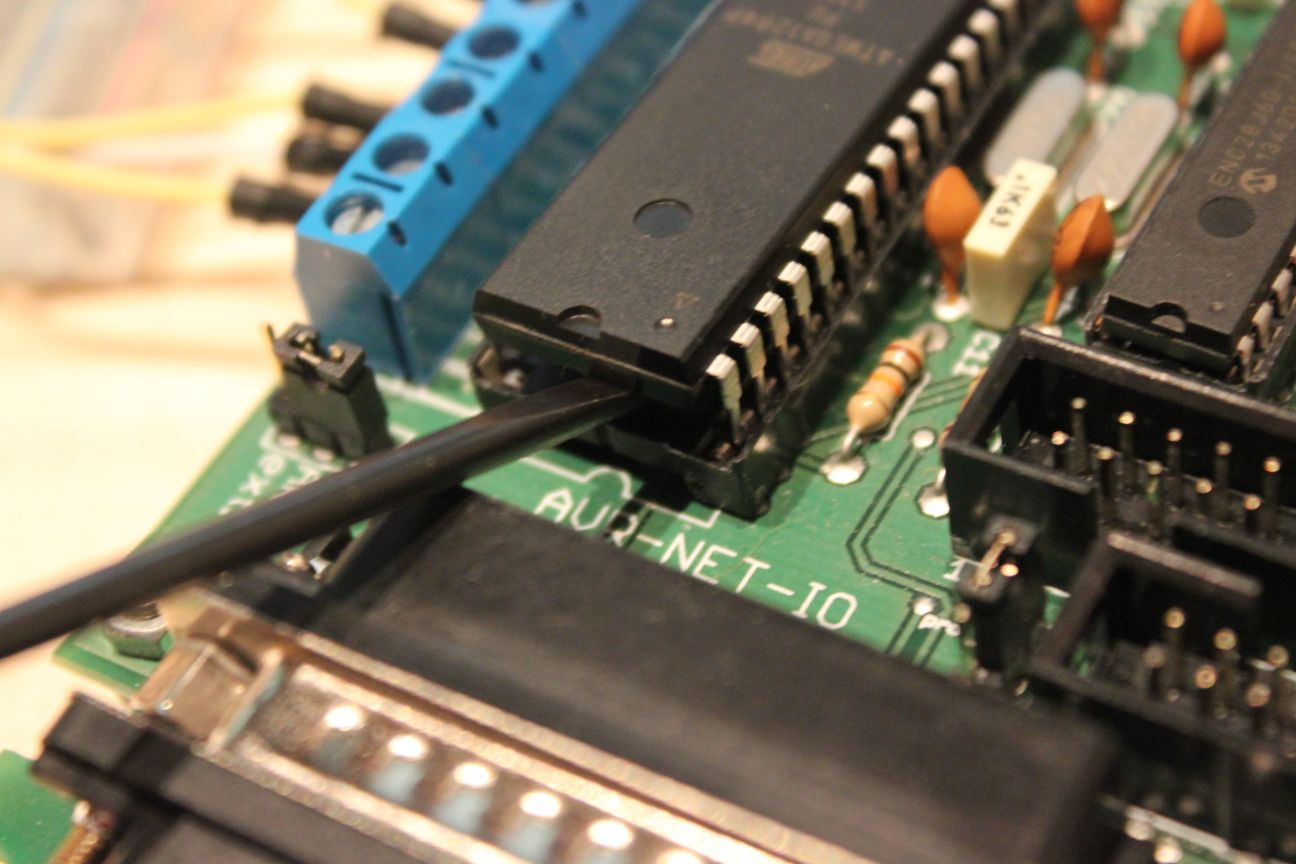
\includegraphics[width=13cm]{content/pictures/Anleitung/tauscheProzessor/1_Hebel.jpg}
\caption{Schraubendreher am Controller}
\label{ausbau1}
\end{figure}

Zum einfachen lösen kann der Hebel auch von der anderen Seite angesetzt
werden. Anschließend den gelösten Prozessor abziehen.

\begin{figure}[H]
\centering
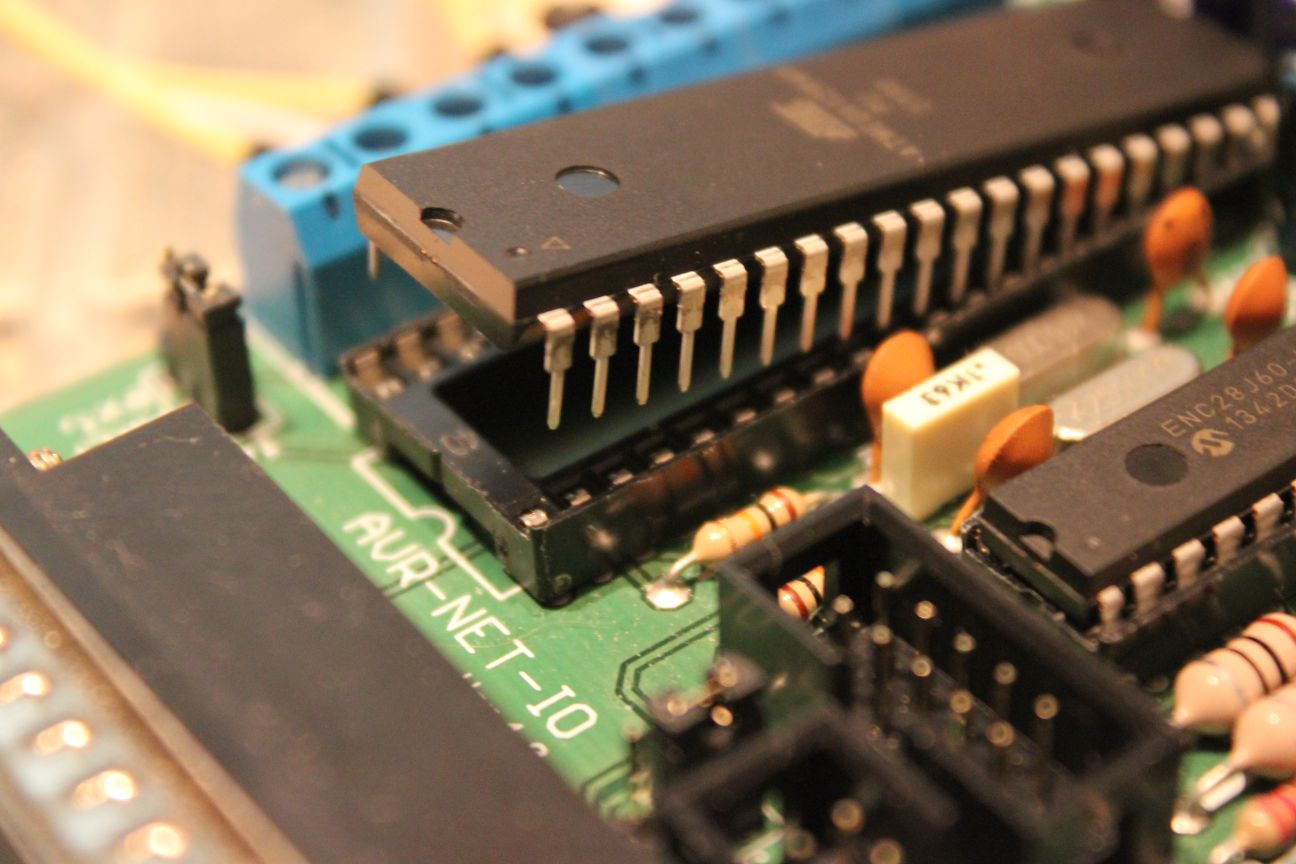
\includegraphics[width=13cm]{content/pictures/Anleitung/tauscheProzessor/2_Geloest.jpg}
\caption{Der gelöste Mikrocontroller}
\label{ausbau2}
\end{figure}

Nachdem der Mikrocontroller entfernt wurde hat man einen guten Blick auf den
Sockel (Abb. \ref{ausbau3}).

\begin{figure}[H]
\centering
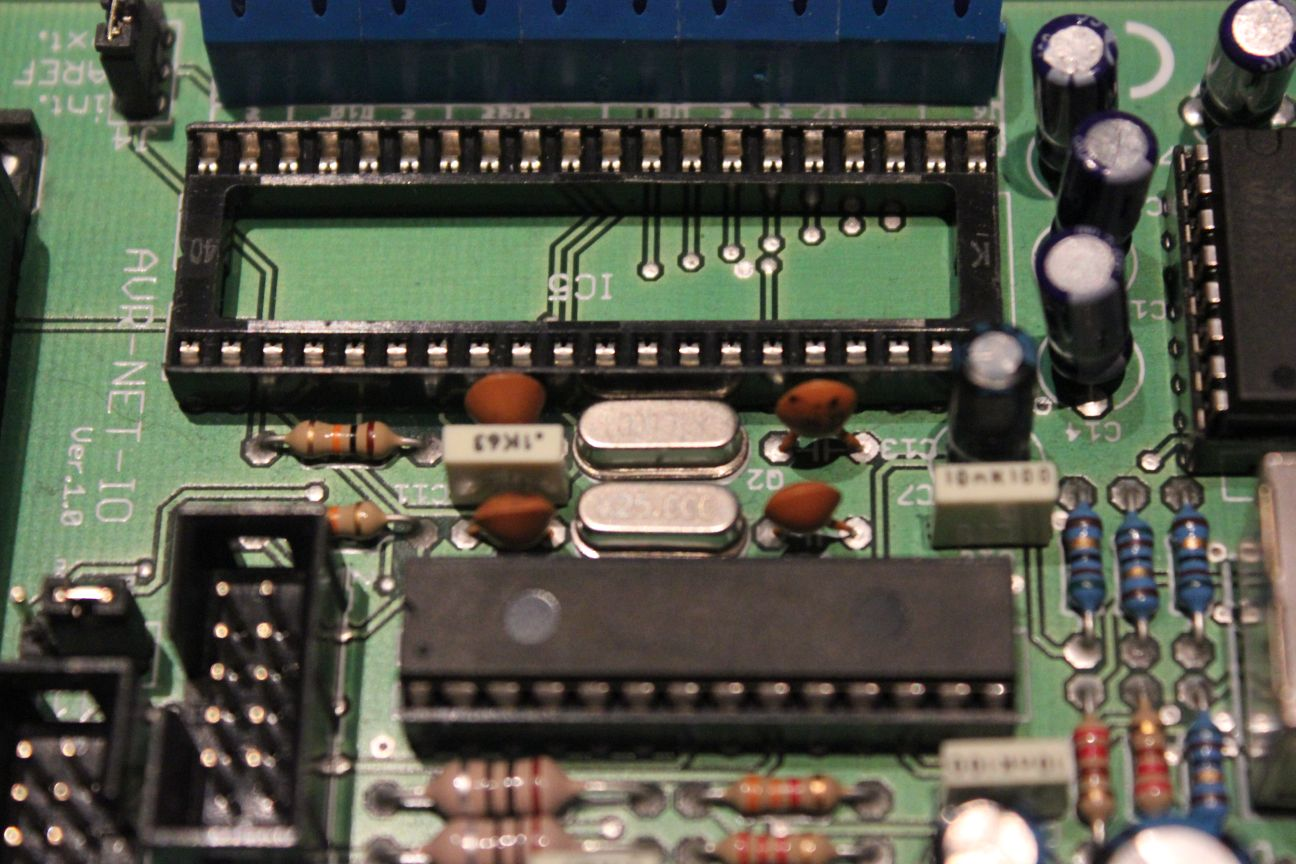
\includegraphics[width=13cm]{content/pictures/Anleitung/tauscheProzessor/3_Sockel.jpg}
\caption{Der Sockel auf dem AVR-Net-IO}
\label{ausbau3}
\end{figure}

Beim Einbau ist unbedingt darauf zu achten den neuen Mikrocontroller entsprechend
der D-Förmige Einkerbung in den Sockel zu setzen. (Siehe Abbildung \ref{ausbau4})

\begin{figure}[H]
\centering
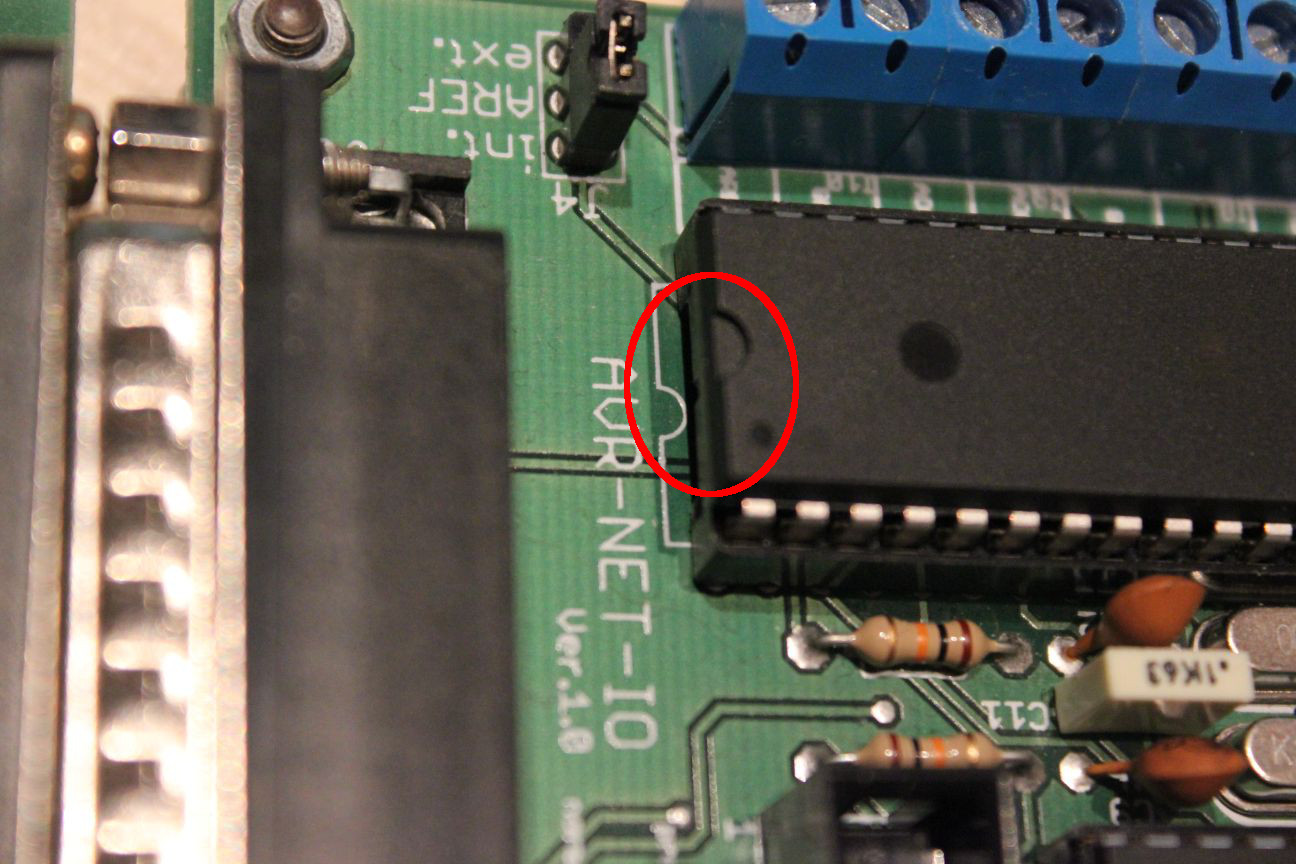
\includegraphics[width=13cm]{content/pictures/Anleitung/tauscheProzessor/4_Markierung.jpg}
\caption{Markierung zum Einbau}
\label{ausbau4}
\end{figure}

\section{ISP-Programmer anschließen}

Der Anschluss des AVRISPmkII Programmers erfolgt über einen 6 Poligen Stecker,
allerdings hat das AVR-Net-IO einen 10 Poligen Stecker. Deswegen wurde hierfür
eigens ein Adapter angefertigt der das ISP Signal von den 6 Polen des Programmers
auf das AVR-Net-IO bring.

\begin{figure}[htp]
\begin{center}
  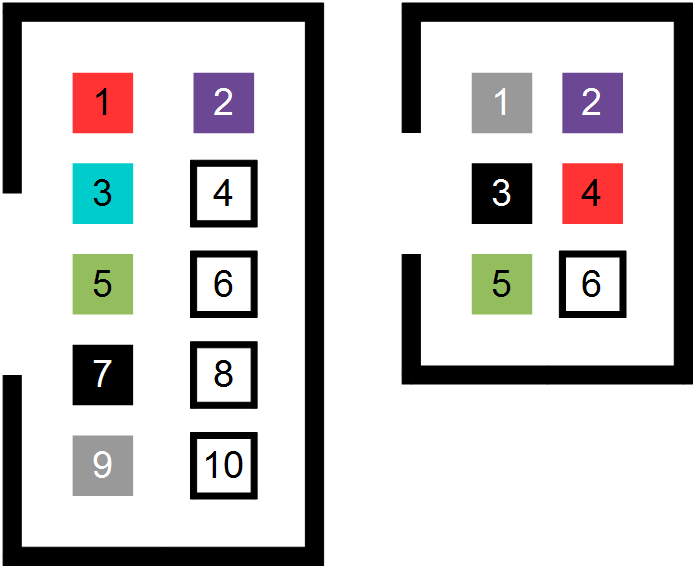
\includegraphics[width=6cm]{content/pictures/Anleitung/ISP-Stecker.png}
  \caption[Schematische Darstellung des ISP Anschlusses]{Schematische Darstellung des ISP Anschlusses (Pin 1 \& 2
  ist auf der Platine markiert)}
  \label{ispanschluss}
\end{center}
\end{figure}

\begin{table}[H]
\centering
\begin{tabular}{|l|l|} \hline
	 \textbf{10-poliger Anschluss} & \textbf{6-poliger Anschluss} \\ \hline
	 1 MOSI & 1 MISO \\ \hline
	 2 VCC & 2 VCC \\ \hline
	 3 - (*) & 3 SCK \\ \hline
	 4,6,8,10 GND & 4 MOSI \\ \hline
	 5 RESET & 5 RESET \\ \hline
	 7 SCK & 6 GND \\ \hline
	 9 MISO &   \\ \hline
\end{tabular}
\caption{Die Pinbelegung für den 6 und 10 poligen Anschluss \cite{mikrocontroller.isp}}
\label{pinbelegung}
\end{table}

\begin{figure}[htp]
\begin{center}
  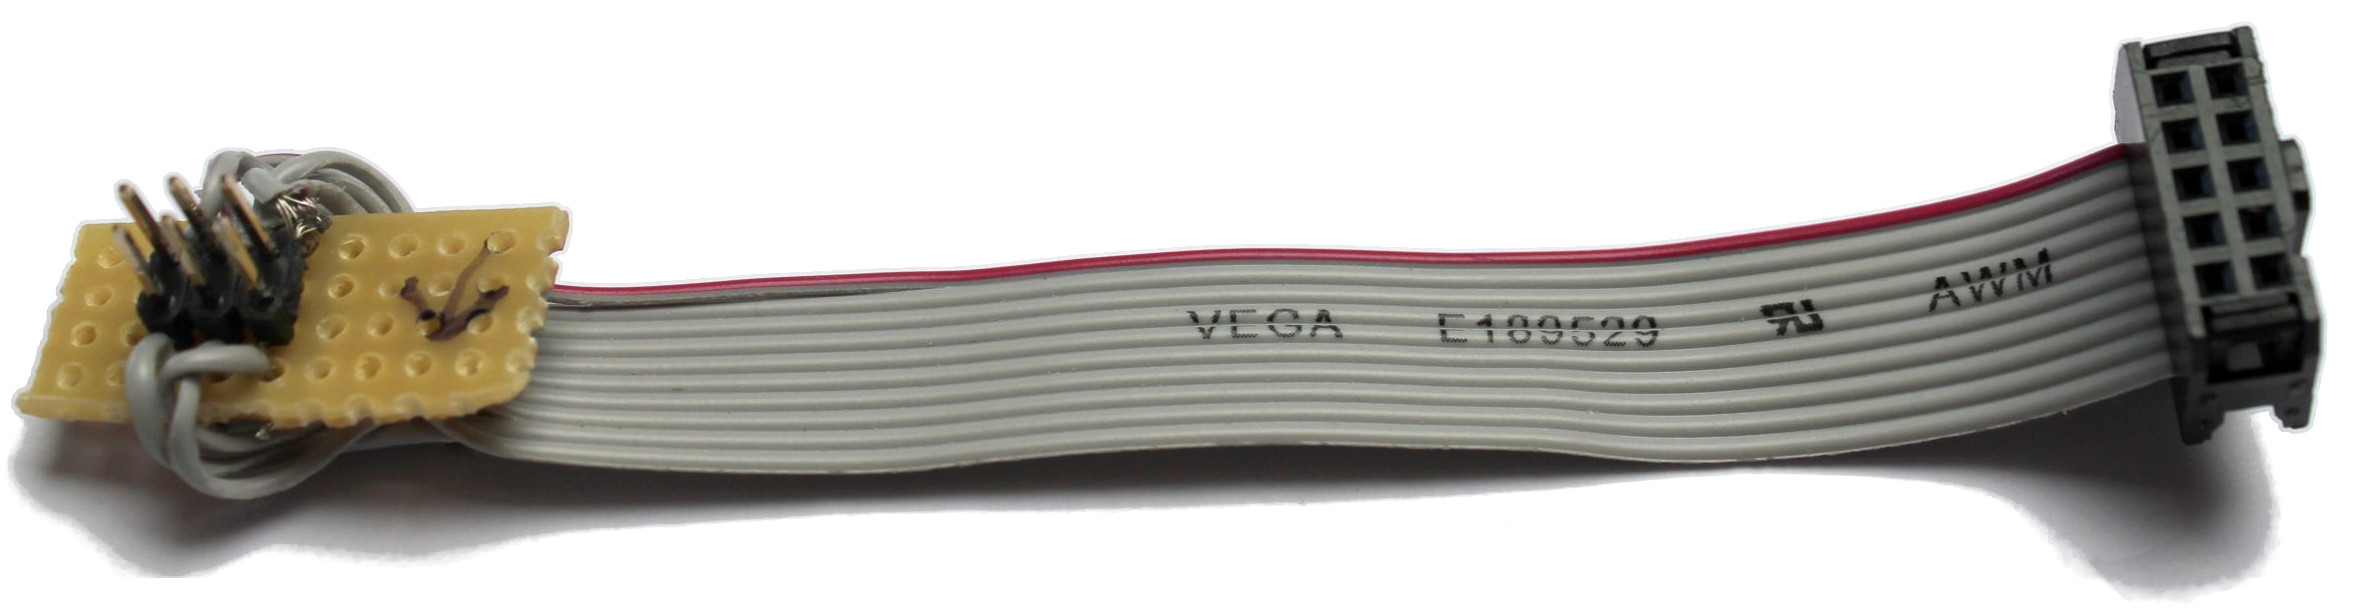
\includegraphics[width=10cm]{content/pictures/Anleitung/adapter.jpg}
  \caption{Der Adapter}
  \label{adapter}
\end{center}
\end{figure}

Mit dem angefertigtem Adapter kann der Debugger anschließend ganz einfach mit
dem Board verbunden werden. Wenn der Mikrocontroller richtig, wie im nächsten Schritt
beschrieben, konfiguriert ist, kann der Programmer auch in Atmel Studio
verwendet werden.

\section{Einrichten eines neuen Mikrocontrollers}

Für einen neuen Chip ist es anfangs notwendig die Fuse-Bits richtig zu setzen,
damit der Chip Ordnungsgemäß Arbeitet.
Dies ist jedoch im AtmelStudio nicht Möglich, da es nicht möglich ist die exakte
Geräte-Signatur auszulesen.
Das Problem liegt darin, das Standartmäßig die Fuses auf den internen
Quarz-Kristall gesetzt sind und nicht auf den Externen Kristall des
AVR-NET-IO Boards.
Beim versuch die Fuse-Bits zu setzen wird man im Atmel Studio mit folgender
Fehlermeldung begrüßt. 
\begin{figure}[h]
\centering
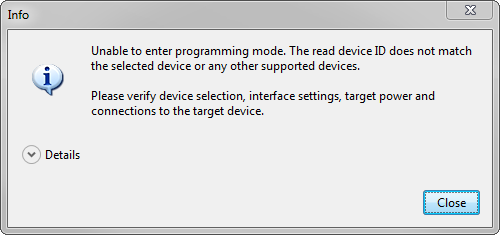
\includegraphics[width=13cm]{content/pictures/Anleitung/neuerProzessor/AnleitungNeuerProzessor2_fehler.png}
\caption{DeviceProgramming}
\end{figure}

Abhilfe Schafft hier die Alternative Programmiersoftware AVRDUDE, mit ihr ist
es Möglich die Fuse-Bits zu ändern. Unter Linux kann dieser einfach über die
Paketquellen installiert werden, für ein Windows Betriebssystem kann eine
ausführbare Kommandozeilen-Anwendung auf der Projekt-Website heruntergeladen
werden \url{http://savannah.nongnu.org/projects/avrdude}. Zusätzlich muss für
Windows noch libusb-win32 (\url{http://sourceforge.net/projects/libusb-win32/})
vorhanden sein, das der Programmer mit den gewählten Parametern verwendet werden
kann. Eine ausführliche Anleitung gibt es hier:
\url{http://eliaselectronics.com/using-the-avrispmkii-with-avrdude-on-windows/}

Die in Folgendem Beispiel angezeigten Befehle sind die von uns verwendeten Fuse
Einstellungen. Für eine genauere Beschreibung wofür die einzelnen Fuse-Bits
verwendet werden, ist der Abschnitt \ref{chap:Fuse} Fusebits im Kapitel 
Hardware.

\begin{table}[H]
\begin{tabular}{| p{.24\textwidth} | p{.76\textwidth} |}
\hline
Auslesen Linux:& sudo avrdude -P usb -p m644p -c avrispmkII  -U lfuse:r:-:h -U hfuse:r:-:h -B 22 \\ \hline
Setzen Linux:& sudo avrdude -P usb -p m644p -c avrispmkII -U lfuse:w:0xFF:m -U hfuse:w:0xD6:m -B 22 \\ \hline
Auslesen Windows:& avrdude.exe -p m644p -c avrispmkII -U lfuse:r:-:h -U hfuse:r:-:h -B 22 \\ \hline 
Setzen Windows:& avrdude.exe -p m644p -c avrispmkII -U lfuse:w:0xFF:m -U hfuse:w:0xD6:m -B 22 \\ \hline
\end{tabular}
\caption{Auslesen und setzen von Fuse-Bits des ATmega644P mit AVRDUDE}
\label{ParameterAvrdude1}
\end{table}

\begin{figure}[h]
\centering
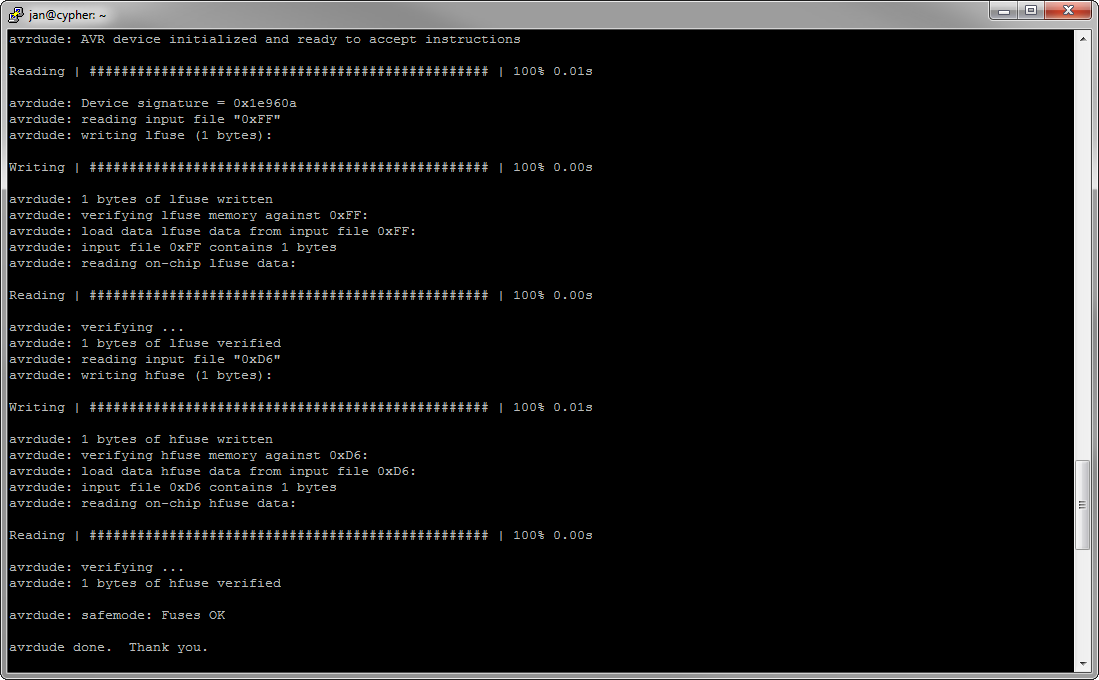
\includegraphics[width=13cm]{content/pictures/Anleitung/neuerProzessor/avrOutput.png}
\caption{AVRDUDE Ausgabe}
\end{figure}

Ein Auszug der verwendeten Parameter aus der AVRDUDE Handbuch Seite:

\begin{table}[H]
\begin{tabular}{| p{.35\textwidth} | p{.65\textwidth} |}
\hline
-p partno & This is the only option that is mandatory for every invocation of
avrdude.  It specifies the type of the MCU connected to the programmer. These
are read from the config file.  If avrdude does not know about a part that you
have, simply add it to the config file (be sure and submit a patch back to the
author so that it can be incorporated for the next version). \newline
\textbf{m32 $\Rightarrow$ ATmega32} \newline 
\textbf{m644p $\Rightarrow$ ATmega644P} \newline
\textbf{m1284p $\Rightarrow$ ATmega1284P} \\ \hline
-P port & Use port to identify the device to which the programmer is attached. \textbf{usb für den AVRISP MKII}  \\ \hline 
-c programmer-id & \textbf{avrispmkII für den AVRISP MKII} \\ \hline
-U \hbox{memtype:op:filename:filefmt} &  
The \textrm{memtype} field specifies the memory type to operate on.\newline
\textbf{hfuse} The high fuse byte.\newline
\textbf{lfuse} The low fuse byte.\newline
The \textrm{op} field specifies what operation to perform:\newline
\textbf{r} read device memory and write to the specified file\newline
\textbf{w} read data from the specified file and write to the device memory \newline
The filename field indicates the name of the file to read or write.  The format field is optional and contains the format of the file to read or write. \newline
\textbf{Hier die Bytes die gesetzt werden 0xFF bzw 0xD6} \\ \hline
-B bitclock & Specify the bit clock period for the JTAG interface or the ISP clock \\ \hline
\end{tabular}
\caption{Auslesen und setzen von Fuse-Bits mit dem AVRDUDE}
\label{parameterAvrdude2}
\end{table}
Anschließend kann der Mikrocontroller zusammen mit dem AV-Net-IO und AtmelStudio
Programmiert werden. Der Verwendete Mikrocontroller wird jetzt richtig erkannt,
da es auch keine Probleme mit der Gerätesignatur gibt.

\section{HTML Header Compiler}
\label{chap:benutzerhandbuch.HHC}

Da der HTML Header Compiler in Java entwickelt wurde muss für die Verwendung die
Java Laufzeitumgebung ab Version 6 installiert sein. Zum Ausführen des Compiler
muss zuerst mit einer Konsole in den Entsprechenden Ordner navigiert werden.
Anschließend kann mit folgendem Befehl die Datei ausgegeben werden. 
\\

\framebox[1.1\width]{java -jar hhc.jar -in <INPUT FOLDER> -out <OUTPUT FILE>} 
\\

Die Angaben in den spitzen Klammern müssen durch den entsprechenden Pfad und
die entsprechende Datei ausgetauscht werden. Standardmäßig optimiert der
HTML Header Compiler die eingegebenen Dateien, falls dies nicht gewünscht ist
gibt es zusätzlich zu den vorgegebenen Optionen weitere Flags
die gesetzt werden können. Hier alle Parameter im Überblick:

\begin{table}[H]
\begin{tabular}{| p{.24\textwidth} | p{.76\textwidth} |}
\hline
-in, -input & Der Eigabepfad mit allen für die Website benötigten Dateien. z.B. \textrm{-in "Webseite"} \\ \hline 
-out, -output & Die Ausgabe Headerdatei z.B. \textrm{-out "Webserver/webpage.h"} \\ \hline
-v, -verbose &  Gibt die ausgegebenen Dateien auf der Console aus. \\  
 \hline 
 -n, -newline & Behält die Formatierung für den Zeilenvorschub, Tabulator
 oder Wagenrücklauf in den HTML und JS Dateien (\textbackslash n and
 \textbackslash r \textbackslash t).
 Benötigt dadurch abhängig von der Website mehr Speicher, ermöglicht aber ein
 einfacheres Debuggen von eingebundenem JavaScript Code.  \\ \hline
\end{tabular}
\caption{Parameter des HTML Header Compiler}
\label{parameterHHC}
\end{table}

Um die Entwicklung zu vereinfachen ist es hilfreich, wenn für den Parameteraufruf
des HTML Header Compilers ein einfaches Schell- oder Batch-Script erstellt, das
die Dateien aus dem Ordner für die Website als Headerdatei in den Ordner für den
Webserver schreibt. Falls eine Änderung an der Website vorgenommen wurde muss
vor dem Programmieren des Mikrocontrollers lediglich der \ac{HHC} Ausgeführt
werden.

\begin{figure}[H]
\lstinputlisting[language=sh]{content/code/buildwebpage.sh}
\caption{BuildWebpage.sh für Linux}
\label{output}
\end{figure}

\begin{figure}[H]
\lstinputlisting[language=sh]{content/code/buildwebpage.bat}
\caption{BuildWebpage.bat für Windows}
\label{output}
\end{figure}

\subsection{Konfiguration des Webservers}

Die Einstellung des Webservers erfolgt über die \textrm{config.h} Datei. In der
\textrm{config.h} Datei, können Zum einen die verschiedenen Pins der Ports als Ein oder
Ausgang definiert werden. Dabei gibt es ein paar Eigenheiten zu beachten:
\begin{itemize}
  \item OUTA steht für den A Port, hier ist du beachten, das dieser Port die
  Analog zu Digital Wandler beherbergt. Mit aktiviertem Wandler ist es nicht
  möglich die Pins des Ports funktionierend als Ausgänge zu schalten, da die
  Spannung nicht gehalten wird.
  \item OUTB ist nur mit Vorsicht zu genießen. Hier handelt es sich um den Port
  der auf dem AVR-Net-IO für die Neztwerkkomunikation genutzt wird. Deswegen
  wird Port B auch nicht Standardmäßig definiert.
  \item OUTC dieser Port wird von Polin standardmäßig für die Ausgänge verwendet
  und ist von uns bereits so Modifiziert. Der gesamte Port wird auf dem
  AVR-NET-IO über den 25Pin D-Sub Stecker geleitet. Wenn der Fuse-Bit für JTag
  geschaltet ist werden 4 Pins des C Ports für das JTag Interface verwendet.
  \item OUTC Der C Port liegt auf dem AVR-Net-IO auf dem EXT Anschluss und ist
  für erweiterte Peripherie geplant, so kann hier ein Cardreader oder ein
  Erweiterungsboard angeschlossen werden.
\end{itemize}
Weiter kann die gewünschte IP-Adresse eingestellt werden, unter der das Gerät
erreicht werden kann. Wichtig ist hier, das kein anderes Gerät die selbe Adresse
im Netzwerk verwendet. Auch kann die Router IP-Adresse und Netzmaske angegeben
werden. Eine weitere Wichtige Einstellung ist die verwendete Mac Adresse
des Netzwerk Controllers. Diese wird über die Variablen MYMAC1-6 Definiert.

\section{Debuggen über JTAG}

Der JTAGICEmkII Debugger von Atmel, den wir für unser Projekt gestellt bekommen
haben, unterstützt neben ISP auch JTAG. Allerdings werden für den Anschluss von
JTAG andere Pins benötigt als für den Anschluss eines ISP Programmers.

%TODO Grafik Pins auf Mikrocontroller zu JTAG

\section{Hexfiles Überspielen}

Zum übertragen der Hexfiles gibt es verschiedene Möglichkeiten.


\subsection{Atmel Studio}

\section{Die Website}
